\chapter{Preliminary Results and Discussion}

\section{Data Exploration} \label{data-exploration} 
Data exploration refers to the process of analyzing, cleaning, transforming, and modeling data with the goal of discovering valuable insights and understanding the underlying structure of the data. It is an essential step in the data science process and involves visualizing and summarizing data, identifying patterns, outliers and anomalies, and checking for missing or duplicate data. Data exploration helps you get a sense of what your data looks like, identify potential problems, and make informed decisions about how to prepare the data for further analysis. By exploring your data, you can gain insights into the relationships and patterns that exist within the data and gain a better understanding of the problem you are trying to solve.

\subsection{Unique Posts} \label{unique-posts}
First we should look at how many unique posts there are. This is important since we want to make sure that we have enough data to work with. After analyzing the data, we can see that there are 660 unique posts. This is a good sign since it means that we have enough data to work with.

\subsection{Post Time Distribution} \label{post-time}
In order to analyze the longetivity of the current topic on stackoverflow, we will plot the time span distribution of all postings as a whole.
\begin{figure}[H]
  \centering
  \noindent  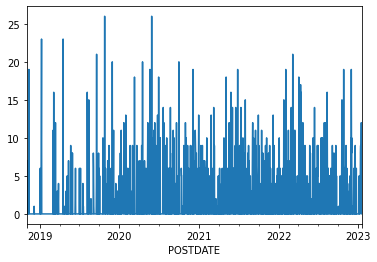
\includegraphics[scale=1]{post-time-distri.png}\\
\caption{Post time distribution}\label{fig:post-time}
\end{figure}

As you can see on the above Figure \ref{fig:post-time}, the number of posts per day is pretty constant. This is a good sign since it means that the number of people using the React UseEffect is still there and therefore it might gives us a better result.

\subsection{Vote Counts Distribution} \label{vote-counts}
Next, we will look at the votecounts distribution across all of the dataset as a whole, it is important to note that the votecounts is the number of votes that a post has received, the higher the votecounts, the more popular the post is. We can probably inference that the more popular the post is, the more likely it is to be answered, and the more likely it is to be answered, the more likely it is to be answered correctly.

\begin{figure}[H]
  \centering
  \noindent 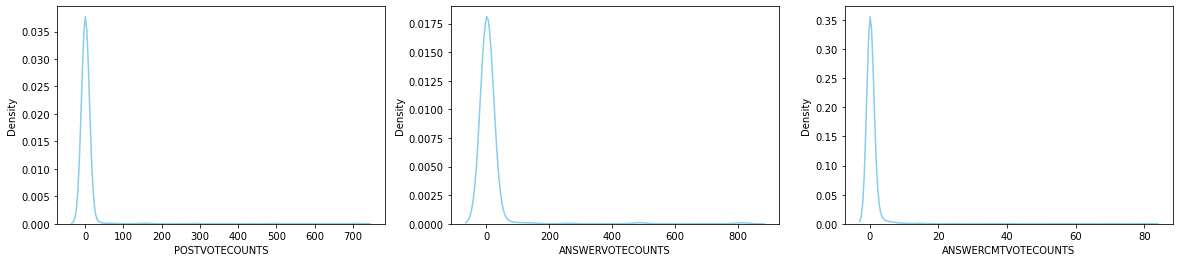
\includegraphics[scale=0.35]{votecounts-distri.png}\\   
\caption{Vote counts distribution}\label{fig:vote-counts}
\end{figure}


As you can tell from the graph in Figure \ref{fig:vote-counts}, the distribution is skewed to the left. This is not a good sign as it means that the majority of the posts have a low votecounts. With that being said, this motivates us to explore more data to be mined from the dataset and facilitate to our work.

% \subsection{Data Cleaning} \label{data-cleaning}
% The scraped data is not perfect. There are some null values that need to be addressed. The following are the null values that need to be addressed:

% \noindent  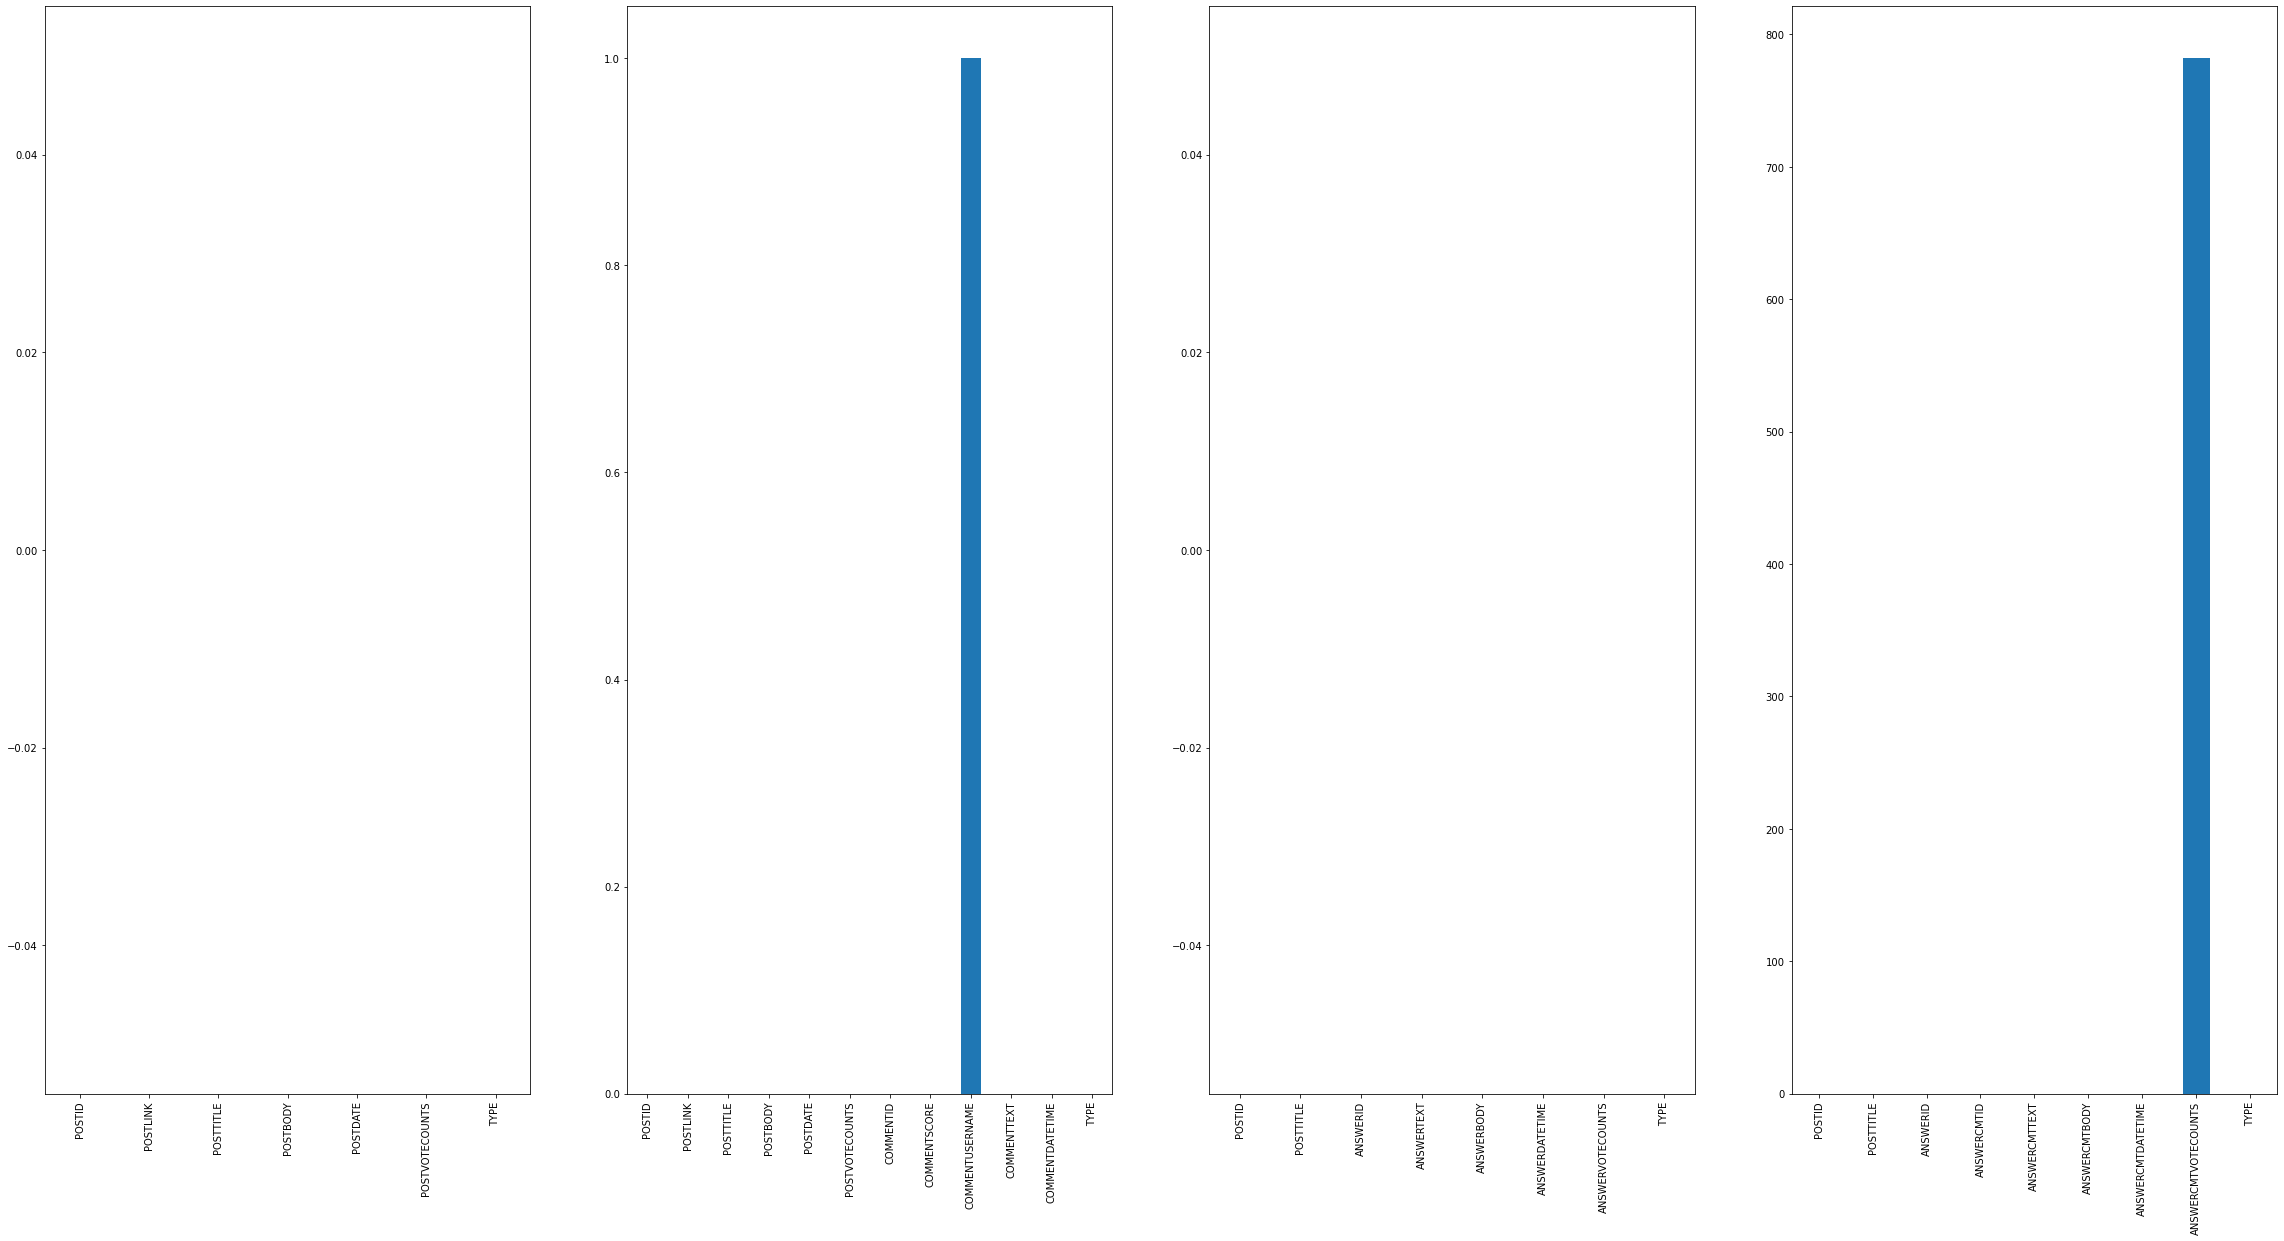
\includegraphics[scale=0.25, angle=90]{null-values-1.png}\\

% From the diagram we can see that everything is perfect except two columns namely the Comment\_Score and Answer\_Comment\_Score. The reason for this is that the comments and answer comments do not have a score. With that being said, we can replace the null values with 0. The following is the result of the replacement:
% 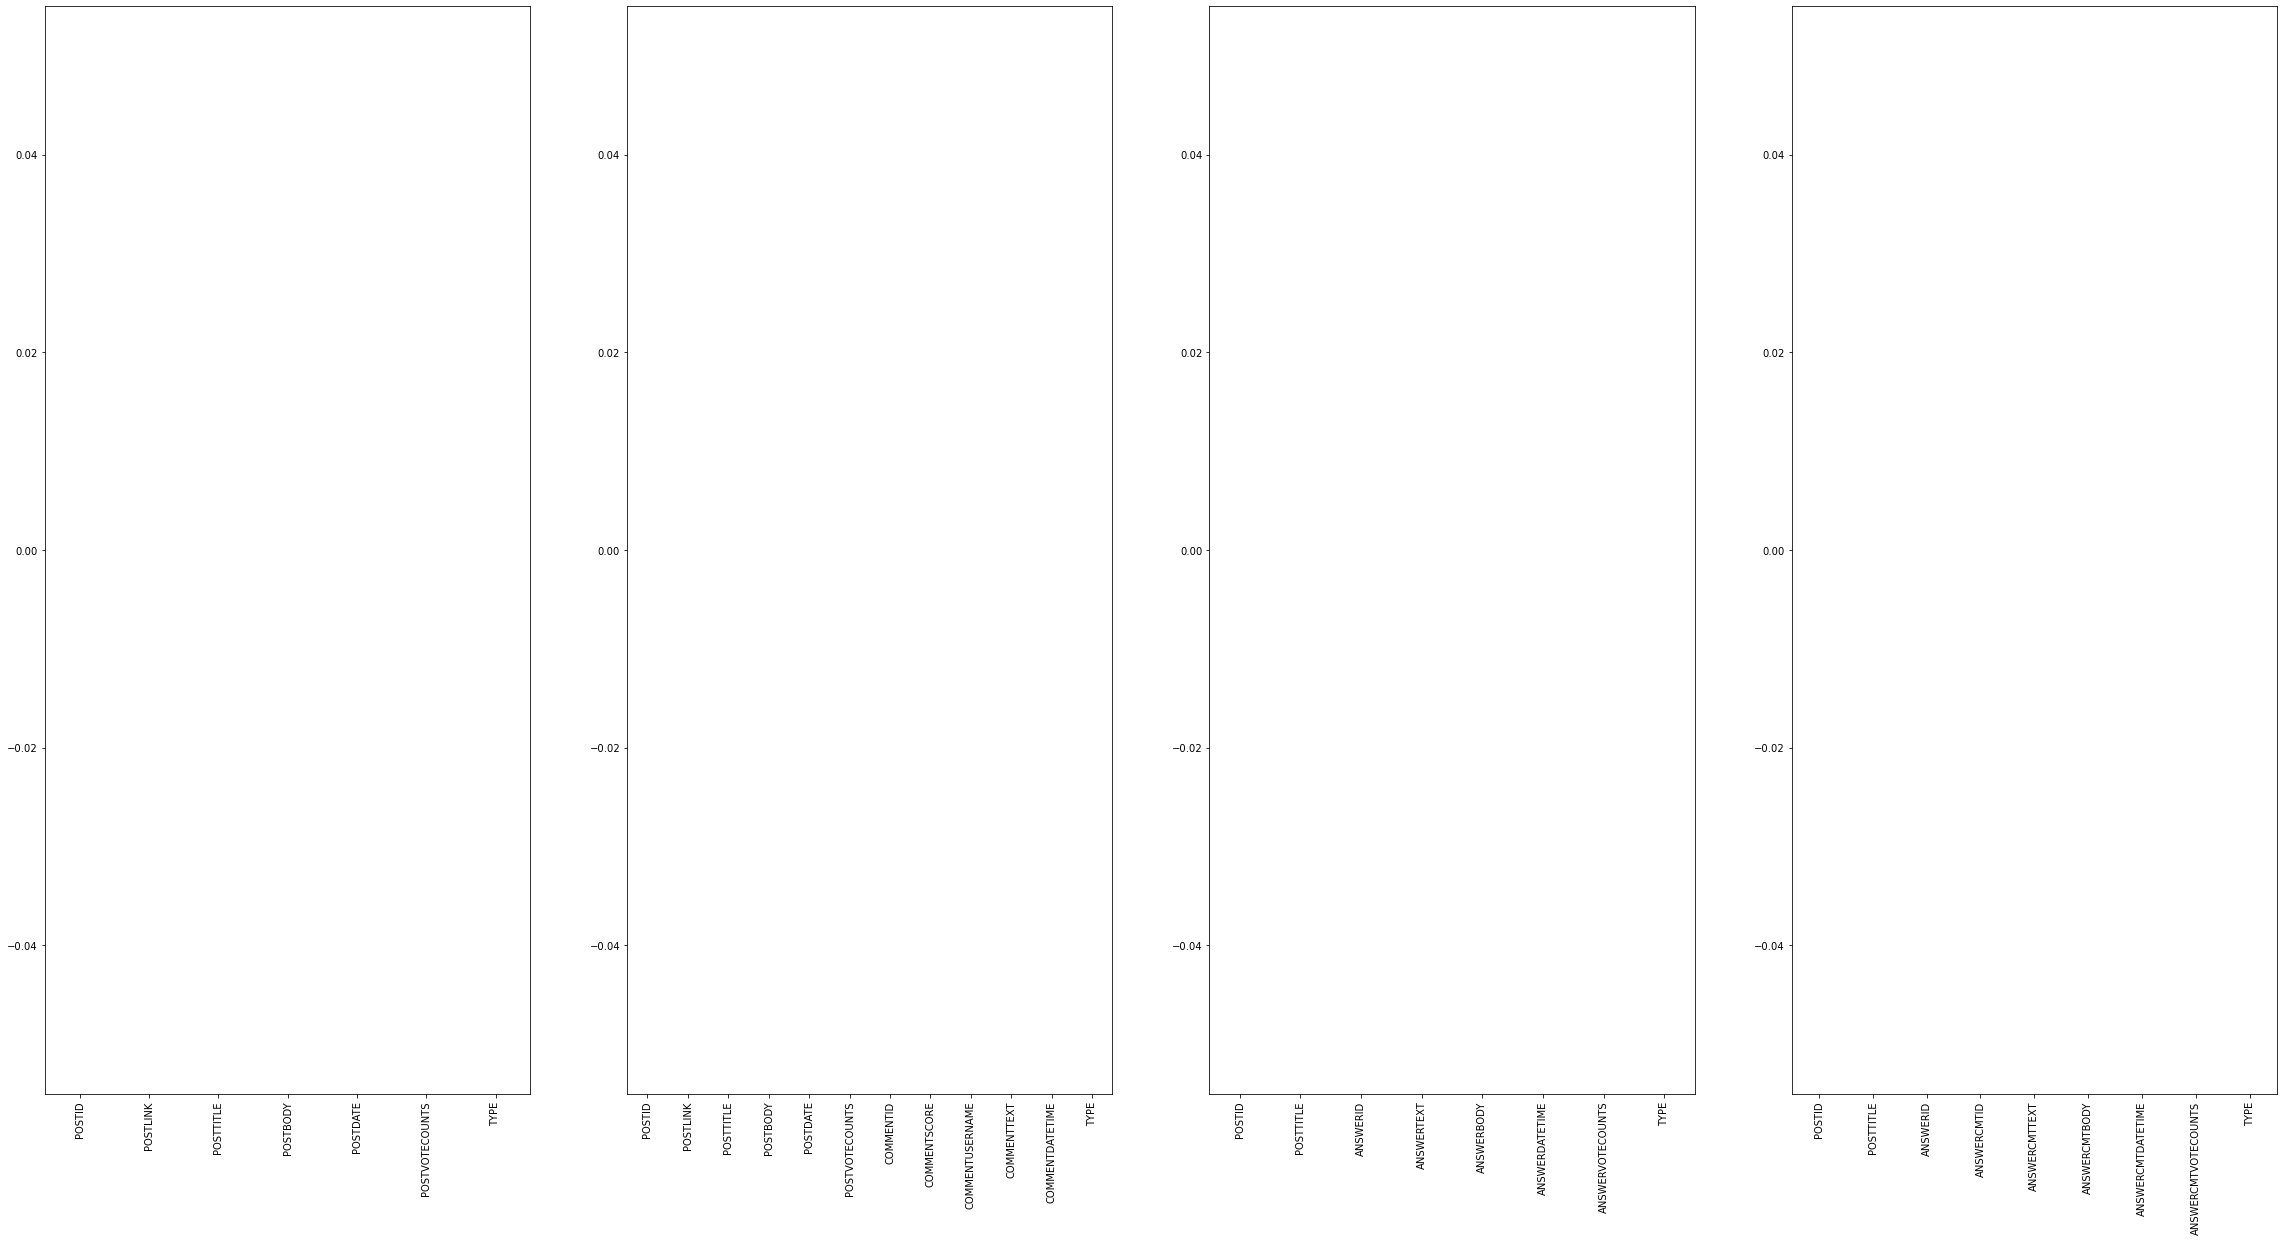
\includegraphics[scale=0.25, angle=90]{null-values-2.png}\\

\section{Post Matching} \label{post-matching_results}
Post Matching is one of the most important part of this work. It is important to note that the post matching is not a trivial task. There are many ways to do it, in the following section we discuss the results that are obtained from 2 different methods that are noted on the "Proposed Framework" section \ref{matching-posts}. In the below discussion, we used the query "How to solve useEffect hook rerenders infinitely?" to test and evaluate the performance of the post matching methods, it is important to note the post's title is the only string that is used to match with the query.

\subsection{Fuzzy Wuzzy: Partial Ratio and Token Sort Ratio Combined} \label{fuzzy-wuzzy_results}
Fuzzy Wuzzy is a python library that provides string matching algorithms. The library provides a simple and efficient way to perform fuzzy string matching tasks, such as finding the similarity ratio between two strings, and finding the closest match for a given string from a list of potential candidates. A detailed discussion on how partial ratio and token sort ratio differ from each other is further highlighted \ref{matching-posts}.

\subsubsection{Resutls:} \label{partial-ratio_results}
\begin{figure}[H]
  \centering
  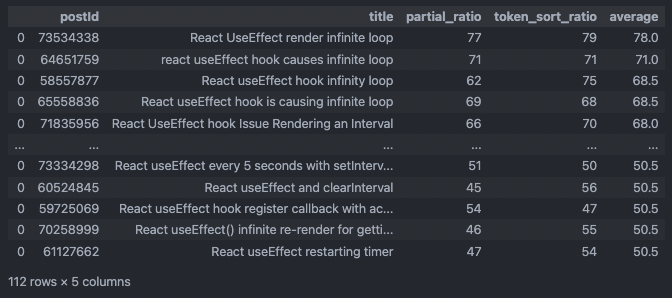
\includegraphics[scale=0.60]{assets/fuzzy-wuzzy-query-1-results.png}
  \caption{Partial Ratio and Token Sort Ratio Combined Results}
  \label{fig:partial-ratio}
\end{figure}

\noindent Using the partial ratio method combined with token sort ratio, it is able to yield 112 posts title to match with the query.

\subsubsection{Spacy Similarity}
Spacy is a python library that provides a lot of NLP tools. The library provides a simple and efficient way to perform NLP tasks, such as finding the similarity ratio between two strings, and finding the closest match for a given string from a list of potential candidates. A detailed discussion on how spacy similarity differs from other methods is further highlighted \ref{spacy_similarity}.

\subsubsection{Results:} \label{spacy-similarity_results}
\begin{figure}[H]
  \centering
  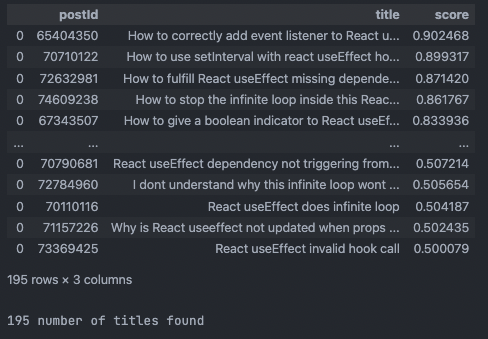
\includegraphics[scale=0.60]{assets/spacy-query-2-results.png}
  \caption{Spacy Results}
  \label{fig:spacy_similarity}
\end{figure}

\noindent A total of 195 posts are matched using the spacy similarity method. Indicating a better matching performance than the fuzzy wuzzy method.

\section{Proprocessing} \label{preprocessing_results}

\subsection{Evaluate Examples} \label{evaluate-examples}

\subsubsection{Example 1} \label{example-1}
\begin{figure}[H]
  \noindent\fbox{%
    \parbox{\textwidth}{%
      Imagine if that was a Web Socket and we were scheduling a new heartbeat tick every time we remounted; the server would be very angry at our apps heart palpitations.
    }%
  }
  \caption{Examples for Evaluation Uses: Example 1}
  \label{fig:example-1}
\end{figure}

\noindent The text above was used to test and evaluate the following sections \ref{stopwords-removal_results} \ref{stemming-vs-lemmatization_results}

\newpage
\subsubsection{Example 2} \label{example-2}
\hspace{0.5cm}
\begin{figure}[H]
  \begin{lstlisting}
'\n<p>You have to convert the response to json <a href="https://google.com">Please Look at this link</a> with await <a href="https://google.com">await</a> response.json();\nand then use setState.</p>\n\n<pre class="lang-js s-code-block"><code class="hljs language-javascript"><span class="hljs-title function_">useEffect</span>(<span class="hljs-function">() =&gt;</span> {         \n        <span class="hljs-variable language_">console</span>.<span class="hljs-title function_">log</span>(<span class="hljs-string">"useEffect TopTen has been called!"</span>);   \n        <span class="hljs-keyword">const</span> <span class="hljs-title function_">fetchdata</span> = <span class="hljs-keyword">async</span> (<span class="hljs-params"></span>) =&gt; {\n        <span class="hljs-keyword">const</span> response = <span class="hljs-keyword">await</span> api.<span class="hljs-title function_">topTen</span>();  <span class="hljs-comment">// this calls axios(url)</span>\n        <span class="hljs-keyword">const</span> responseData = <span class="hljs-keyword">await</span> response.<span class="hljs-title function_">json</span>();\n </pre>\n    '
        \end{lstlisting}
  \caption{Examples for Evaluation Uses: Example 2}
  \label{fig:example-2}
\end{figure}


\noindent The text shown is a non-edited scraped html from stackoverflow. It was used to evaluate the following sections \ref{extracting-url_results} \ref{code-blocks-removal_results} \ref{html-tags-removal_results}

\subsection{Stopwords Removal} \label{stopwords-removal_results}
Stopwords are identified as the common words that exists in a language, they are usually removed from the text to give more importance to other words in the text. Stopwords lists can be subjective, stopwords list differ itself from one language to another, also they are different when treating texts from different domains. A detailed discussion on this domain is further highlighted \ref{sssec:preprocessing_finding_tech_related_stop_words}.

\subsubsection{Results:} \label{stopwords-removal_results_results}
The results after using the stopwords removal is as follows:

\begin{figure}[H]
  \begin{center}
    \begin{tabular}{|p{9cm}|p{5cm}|}
    \hline\hline
    Original & Results \\ [0.5ex] % 
    \hline 
    Imagine if that was a Web Socket and we were scheduling a new heartbeat tick every time we remounted; the server would be very angry at our apps heart palpitations. & imagine web socket scheduling new heartbeat tick every time remounted; server would angry apps heart palpitations.  \\ 
    \hline 
    \end{tabular}
  \end{center}
  \caption{Stopwords Removal Results}
  \label{fig:stopwords-removal_results}
\end{figure}

\hspace{1cm}

\subsection{Stemming vs Lemmatization} \label{stemming-vs-lemmatization_results}
A comparison of the results of stemming and lemmatization is shown below. Stemming is the process of reducing inflected (or sometimes derived) words to their word stem, base or root form—generally a written word form. Lemmatization is the process of grouping together the inflected forms of a word so they can be analysed as a single item, identified by the word's lemma, or dictionary form. A detailed discussion on this domain is further highlighted \ref{sssec:preprocessing_lemmatization_stemming}.

\subsubsection{Stemming Results:} \label{stemming-vs-lemmatization_results_results_2}
\begin{figure}[H]
  \begin{center}
    \begin{tabular}{|p{9cm}|p{5cm}|}
    \hline\hline
    Original & Results \\ [0.5ex] % 
    \hline 
    Imagine if that was a Web Socket and we were scheduling a new heartbeat tick every time we remounted; the server would be very angry at our apps heart palpitations. & imagin if that wa a web socket and we were schedul a new heartbeat tick everi time we remount ; the server would be veri angri at our app heart palpit .  \\ 
    \hline 
    \end{tabular}
  \end{center}
  \caption{Stemming Results}
  \label{fig:stemming-vs-lemmatization_results_results_2}
\end{figure}

\subsubsection{Lemmatization Results:} \label{stemming-vs-lemmatization_results_results_1}
\begin{figure}[H]
  \begin{center}
    \begin{tabular}{|p{9cm}|p{5cm}|}
    \hline\hline
    Original & Results \\ [0.5ex] % 
    \hline 
    Imagine if that was a Web Socket and we were scheduling a new heartbeat tick every time we remounted; the server would be very angry at our apps heart palpitations. & Imagine if that wa a Web Socket and we were scheduling a new heartbeat tick every time we remounted ; the server would be very angry at our apps heart palpitation .  \\ 
    \hline 
    \end{tabular}
  \end{center}
  \caption{Lemmatization Results}
  \label{fig:stemming-vs-lemmatization_results_results_1}
\end{figure}

\noindent In this work, lemmatization is chosen. Lemmatization has proven to be more effective than stemming if context of the text is taken into consideration. 

\subsection{Extracting URL} \label{extracting-url_results}
\subsubsection{Results:} \label{extracting-url_results_results}

\newpage
\begin{figure}[H]
  \begin{center}
    \begin{tabular}{|p{8cm}|p{6cm}|}
    \hline\hline
    Original & Extracted \\ [0.5ex] % 
    \hline 
    \begin{lstlisting}[frame=none]
'\n<p>You have to convert the response to json <a href="https://google.com">Please Look at this link</a> with await <a href="https://google.com">await</a> response.json();\nand then use setState.</p>\n\n<pre class="lang-js s-code-block"><code class="hljs language-javascript"><span class="hljs-title function_">useEffect</span>(<span class="hljs-function">() =&gt;</span> {         \n        <span class="hljs-variable language_">console</span>.<span class="hljs-title function_">log</span>(<span class="hljs-string">"useEffect TopTen has been called!"</span>);   \n        <span class="hljs-keyword">const</span> <span class="hljs-title function_">fetchdata</span> = <span class="hljs-keyword">async</span> (<span class="hljs-params"></span>) =&gt; {\n        <span class="hljs-keyword">const</span> response = <span class="hljs-keyword">await</span> api.<span class="hljs-title function_">topTen</span>();  <span class="hljs-comment">// this calls axios(url)</span>\n        <span class="hljs-keyword">const</span> responseData = <span class="hljs-keyword">await</span> response.<span class="hljs-title function_">json</span>();\n </pre>\n    '
    \end{lstlisting} & [('https://google.com', 'Please Look at this link'), ('https://google.com', 'await')] \\ 
  
    \hline 
    \end{tabular}
  \end{center}
  \caption{Extracting URL Results}
  \label{fig:extracting-url_results_results}
\end{figure}

The url and the text that is linked to the url is extracted and shown in the results.

\subsection{Code Blocks Removal } \label{code-blocks-removal_results}
\subsubsection{Results:} \label{code-blocks-removal_results_results}
\newpage
\begin{figure}[H]
  \begin{center}
    \begin{tabular}{|p{8cm}|p{6cm}|}
    \hline\hline
    Original & Results \\ [0.5ex] % 
    \hline 
    \begin{lstlisting}[frame=none]
'\n<p>You have to convert the response to json <a href="https://google.com">Please Look at this link</a> with await <a href="https://google.com">await</a> response.json();\nand then use setState.</p>\n\n<pre class="lang-js s-code-block"><code class="hljs language-javascript"><span class="hljs-title function_">useEffect</span>(<span class="hljs-function">() =&gt;</span> {         \n        <span class="hljs-variable language_">console</span>.<span class="hljs-title function_">log</span>(<span class="hljs-string">"useEffect TopTen has been called!"</span>);   \n        <span class="hljs-keyword">const</span> <span class="hljs-title function_">fetchdata</span> = <span class="hljs-keyword">async</span> (<span class="hljs-params"></span>) =&gt; {\n        <span class="hljs-keyword">const</span> response = <span class="hljs-keyword">await</span> api.<span class="hljs-title function_">topTen</span>();  <span class="hljs-comment">// this calls axios(url)</span>\n        <span class="hljs-keyword">const</span> responseData = <span class="hljs-keyword">await</span> response.<span class="hljs-title function_">json</span>();\n </pre>\n    '
    \end{lstlisting} &\begin{lstlisting}[frame=none]
'\n<p>You have to convert the response to json <a href="https://
google.com">Please Look at this link</a> with await <a href="
https://google.com">
await</a> response.json();\n
and then use 
setState.</p>\n\n<pre class="lang-js 
 s-code-block"></pre>\n    '
    \end{lstlisting} \\ 
    \hline 
    \end{tabular}
  \end{center}
  \caption{Code Blocks Removal Results}
  \label{fig:code-blocks-removal_results_results}
\end{figure}

\noindent In this step, the codeblocks is removed from the original html by detecting the tags and classes used.

\subsection{HTML Tags Removal} \label{html-tags-removal_results}
\subsubsection{Results:} \label{html-tags_results_results}
\newpage
\begin{figure}[H]
  \begin{center}
    \begin{tabular}{|p{8cm}|p{6cm}|}
    \hline\hline
    Original & Results \\ [0.5ex] % 
    \hline 
    \begin{lstlisting}[frame=none]
'\n<p>You have to convert the response to json <a href="https://google.com">Please Look at this link</a> with await <a href="https://google.com">await</a> response.json();\nand then use setState.</p>\n\n<pre class="lang-js s-code-block"><code class="hljs language-javascript"><span class="hljs-title function_">useEffect</span>(<span class="hljs-function">() =&gt;</span> {         \n        <span class="hljs-variable language_">console</span>.<span class="hljs-title function_">log</span>(<span class="hljs-string">"useEffect TopTen has been called!"</span>);   \n        <span class="hljs-keyword">const</span> <span class="hljs-title function_">fetchdata</span> = <span class="hljs-keyword">async</span> (<span class="hljs-params"></span>) =&gt; {\n        <span class="hljs-keyword">const</span> response = <span class="hljs-keyword">await</span> api.<span class="hljs-title function_">topTen</span>();  <span class="hljs-comment">// this calls axios(url)</span>\n        <span class="hljs-keyword">const</span> responseData = <span class="hljs-keyword">await</span> response.<span class="hljs-title function_">json</span>();\n </pre>\n    '
    \end{lstlisting} &\begin{lstlisting}[frame=none]
'\nYou have to convert the response to json Please Look at this link with await await response.json();\nand then use setState.\n\nuseEffect(() =&gt; {         \n        console.log("useEffect TopTen has been called!");   \n        const fetchdata = async () =&gt; {\n        const response = await api.topTen();  // this calls axios(url)\n        const responseData = await response.json();\n        setLoading(false);\n        setTopten(responseData.
data);    \n        setError(responseData.
error);    \n    };\n\n    fetchdata ();     \n}, []);\n\n    '
    \end{lstlisting} \\ 
    \hline 
    \end{tabular}
  \end{center}
  \caption{HTML Tags Removal Results}
  \label{fig:html-tags-removal_results_results}
\end{figure}

\noindent In this step, the html tags is removed from the original html by detecting the tags.

\subsection{Combining all proprocessing techniques} \label{combining-all-the-methods-used_results}
By combining all of the proprocessing techinques used above \ref{stopwords-removal_results} \ref{stemming-vs-lemmatization_results} \ref{extracting-url_results} \ref{code-blocks-removal_results} \ref{html-tags-removal_results}, an evaluation is made using Example 2 \ref{example-2}
\newpage
\begin{figure}[H]
  \begin{center}
    \begin{tabular}{|p{8cm}|p{6cm}|}
    \hline\hline
    Original & Results \\ [0.5ex] % 
    \hline 
    \begin{lstlisting}[frame=none]
'\n<p>You have to convert the response to json <a href="https://google.com">Please Look at this link</a> with await <a href="https://google.com">await</a> response.json();\nand then use setState.</p>\n\n<pre class="lang-js s-code-block"><code class="hljs language-javascript"><span class="hljs-title function_">useEffect</span>(<span class="hljs-function">() =&gt;</span> {         \n        <span class="hljs-variable language_">console</span>.<span class="hljs-title function_">log</span>(<span class="hljs-string">"useEffect TopTen has been called!"</span>);   \n        <span class="hljs-keyword">const</span> <span class="hljs-title function_">fetchdata</span> = <span class="hljs-keyword">async</span> (<span class="hljs-params"></span>) =&gt; {\n        <span class="hljs-keyword">const</span> response = <span class="hljs-keyword">await</span> api.<span class="hljs-title function_">topTen</span>();  <span class="hljs-comment">// this calls axios(url)</span>\n        <span class="hljs-keyword">const</span> responseData = <span class="hljs-keyword">await</span> response.<span class="hljs-title function_">json</span>();\n </pre>\n    '
    \end{lstlisting} &\begin{lstlisting}[frame=none]
You have to convert the response to json with await response.json();and then use setState. 
    \end{lstlisting} \\ 
    \hline 
    \end{tabular}
  \end{center}
  \caption{Combining all the methods used}
  \label{fig:combining-all-the-methods-used_results}
\end{figure}

The preprocessing techniques used above has removed the html tags, codeblocks, stopwords, and lemmatized the text. The text is now ready to be used for the following pipeline

\section{Sentence Scoring} \label{sentence-scoring_results}
In order to rank sentences in a document, sentence scoring is used in this work, the mechanics used to achieve such scoring is highlighted in \ref{sssec:preprocessing_sentence_scoring}. The results of the sentence scoring is shown below:

\subsection{Sentence Scoring Results:} \label{sentence-scoring_results_results}
\begin{figure}[H]
  \centering
  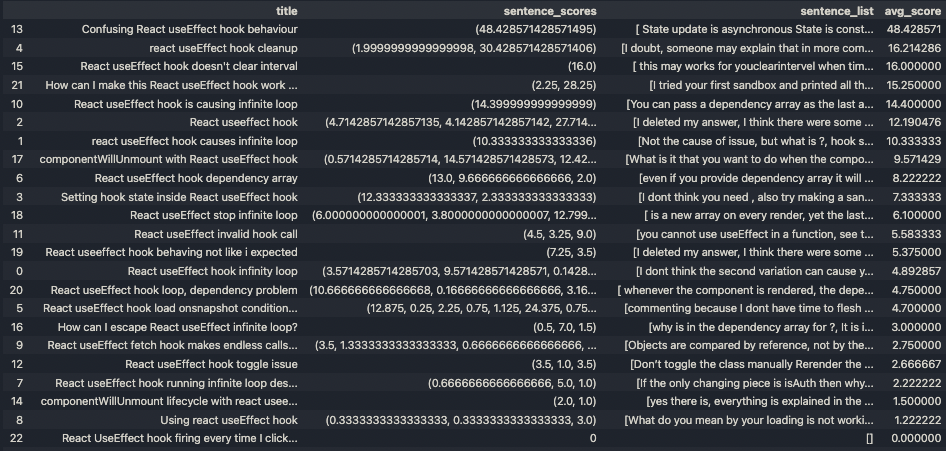
\includegraphics[scale=0.65, angle=90]{assets/sentence-scoring.png}
  \caption{Sentence Scoring Results}
  \label{fig:sentence-scoring}
\end{figure}

The Figure \ref{sentence-scoring_results_results} angled at 90 degrees, shows the result of the sentence scoring algorithm that we've implemented, the average score of all the sentences on a post are located at the far right of the table. Consequently, the posts are ranked based on the average score column.

\section{Rank Posts: Part 1} \label{rank-posts_1_results}
According to the framework proposed in \ref{framework}, the rankings can be evaluated after the sentence scoring is done. The results can be evaluated by using a wordcloud to determine the most important words in selected posts. The wordcloud is shown below:

\begin{figure}[H]
  \centering
  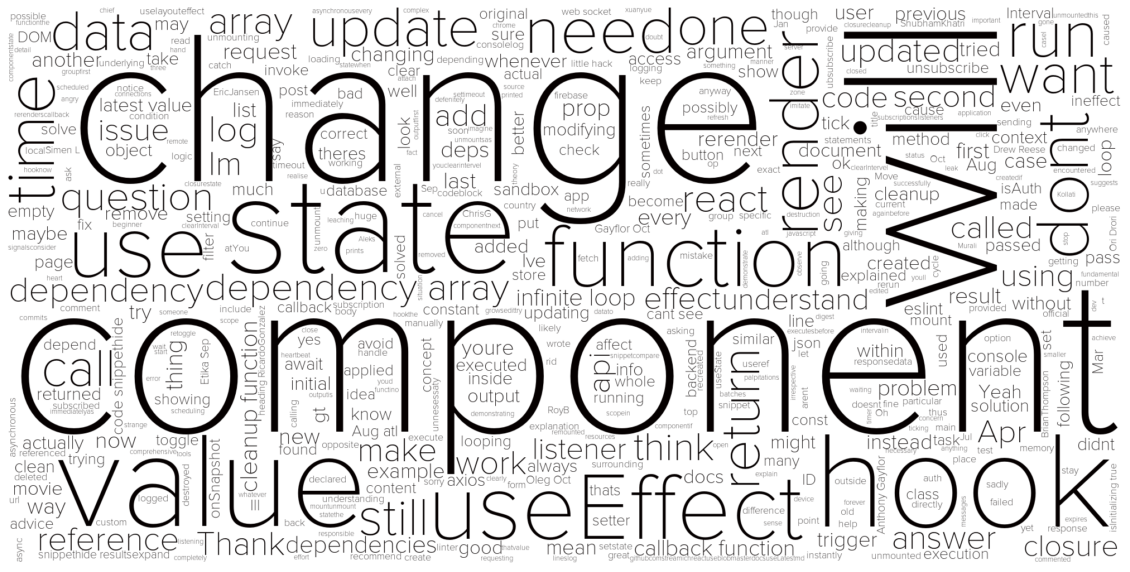
\includegraphics[scale=0.35]{rank_post_1.png}
  \caption{Word Cloud 1st Post Ranking  Results}
  \label{fig:rank_post_1_wc}
\end{figure}

\noindent The word cloud generated this round is quite messy, the important keywords are quite a few, this indicates that the ranking framework is not effective enough. This is expected as the ranking framework is still in its early stages.

\section{Sentiment Analysis} \label{sentiment-analysis_results}
To further rank the sentences, sentiment is another factor that can provide usefull pieces of information to rank the sentences, \ref{sssec:preprocessing_sentiment_analysis}. Note that the list of posts are being filtered in the previous step \ref{sentence-scoring_results}, the filtering basically filters out any posts that have a negative or nan score on the previous step.

\subsection{Sentiment Analysis Results:} \label{sentiment_analysis_results}
\begin{figure}[H]
  \centering
  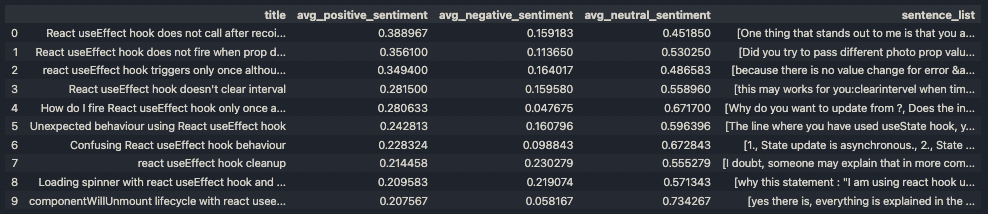
\includegraphics[scale=0.60, angle=90]{assets/sentiment_analysis.png}
  \caption{Sentiment Anlysis Results}
  \label{fig:sentiment-analysis}
\end{figure}

The Figure \ref{fig:sentiment-analysis} angled at 90 degrees, shows the result of the sentiment analysis, the averages of positive, negative, and neutral scores are located at the middle of the table. The posts are ranked based on the average positive score column.

\section{Rank Posts: Part 2} \label{rank-posts_2_results}
The wordcloud is shown below:

\begin{figure}[H]
  \centering
  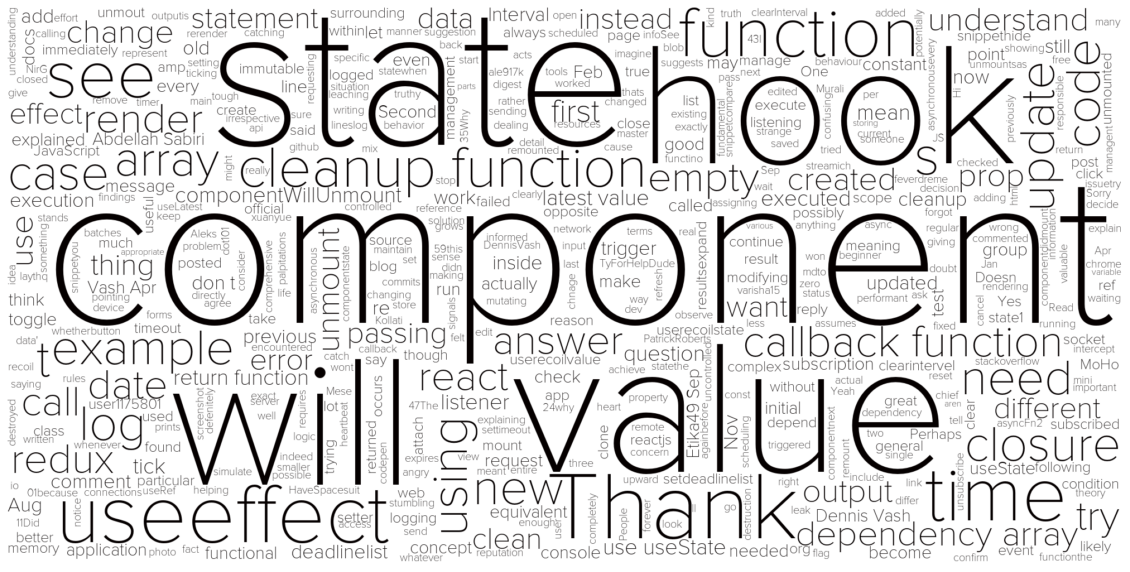
\includegraphics[scale=0.35]{assets/rank_post_2.png}
  \caption{Word Cloud 2nd Post Ranking  Results}
  \label{fig:rank_post_2_wc}
\end{figure}

\noindent The word cloud generated on this section suggests that the important words from the first posts are slighly more exagerated in the second post. This is a good indication of the effectiveness of the ranking system, because the unrelated posts are removed and the related posts are ranked higher.

\section{Summarization} \label{summarization_results}
The final step is to summarize the top 5 posts ranked by the previous step \ref{sentiment-analysis_results}. The detailed explaination of the summarization process and the model used is noted in \ref{sssec:preprocessing_summarization}

\subsection{Summarization Results:} \label{summarization_results}
\begin{figure}[H]
  \centering
  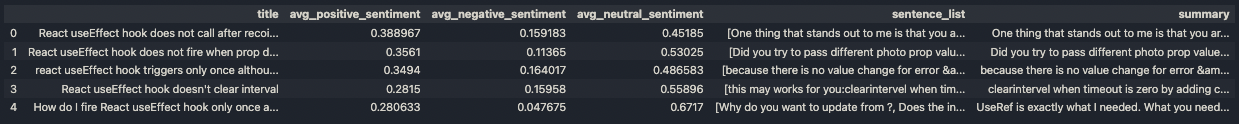
\includegraphics[scale=0.40, angle=90]{assets/summarization.png}
  \caption{Summarization Results}
  \label{fig:summarization}
\end{figure}

The Figure \ref{fig:summarization} angled at 90 degrees, shows the result of the summarization implementation, the summary of the top 5 posts are located at the far right of the table.

\section{Rank Posts: Part 3} \label{rank-posts_3_results}
The wordcloud is shown below:

\begin{figure}[H]
  \centering
  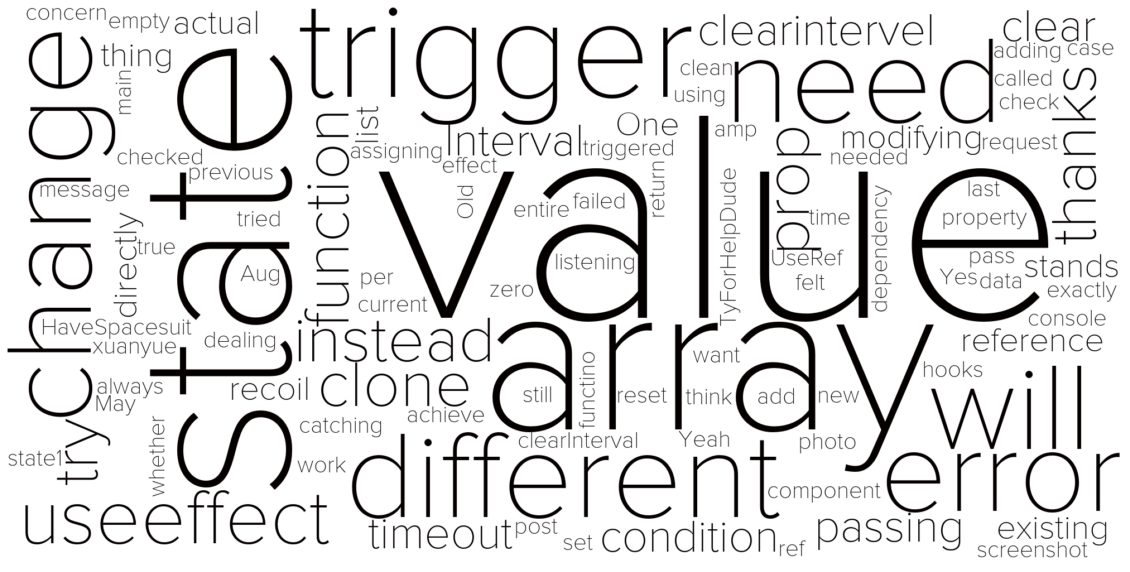
\includegraphics[scale=0.35]{assets/rank_post_3.png}
  \caption{Word Cloud 3rd Post Ranking  Results}
  \label{fig:rank_post_3_wc}
\end{figure}

\noindent The final word cloud gives us a more clearer view on the most important words in the top 5 posts, the words chosen are definitely less noisy than the previous wordclouds.

\section{Survey} \label{survey_results}
The survey is conducted to determine the effectiveness of the system, the survey is conducted on 3 people, 3 of them are experts in the field of "react useeffect" which is the topic of the dataset scraped from stackoverflow. The survey is conducted by asking the experts to come up with the query related to the topic "react useeffect" and to determine if the results of the framework is relevant to the topic of the question and if they're useful to the experts. The results of the survey is shown below:

\subsection{Expert 1} \label{survey_expert_1}
The query asked by expert 1 is:

\begin{figure}[H]
\noindent\begin{lstlisting}
  How to fetch data using the useEffect Hook?
\end{lstlisting}
\caption{Query asked by expert 1}
\label{fig:query-asked-by-expert-1}
\end{figure}

Feedback from expert 1:

\begin{figure}[H]
\noindent\begin{lstlisting}
  The result is relevant to the question, but the summarized output is not useful.
\end{lstlisting}
\caption{Feedback from expert 1}
\label{fig:feedback-from-expert-1}
\end{figure}

\subsection{Expert 2} \label{survey_expert_2}
The query asked by expert 2 is:
\begin{figure}[H]
\noindent\begin{lstlisting}
  useEffect hook doesn't work!
\end{lstlisting}
\caption{Query asked by expert 2}
\label{fig:query-asked-by-expert-2}
\end{figure}

Feedback from expert 2:
\begin{figure}[H]
\noindent\begin{lstlisting}
  It is able to find the post that are related to my prompt.
\end{lstlisting}
\caption{Feedback from expert 2}
\label{fig:feedback-from-expert-2}
\end{figure}

\subsection{Expert 3} \label{survey_expert_3}
The query asked by expert 3 is:

\begin{figure}[H]
\noindent\begin{lstlisting}
  How do i use the Use effect hook with use state.
\end{lstlisting}
\caption{Query asked by expert 3}
\label{fig:query-asked-by-expert-3}
\end{figure}

Feedback from expert 3:
\begin{figure}[H]
\noindent\begin{lstlisting}
  Maybe my query is abit out of context because useState is involved, but surprisingly the framework is able to find the post.
\end{lstlisting}
\caption{Feedback from expert 3}
\label{fig:feedback-from-expert-3}
\end{figure}

